\documentclass[]{jsarticle}
\usepackage[dvipdfmx]{graphicx}

\begin{document}
\title{2SK2936の実験}
\author{青木翔平}
\date{29, Jul 2015}
\maketitle

\section{オシロスコープでの出力波形計測}


\begin{figure}[htbp]
\centering
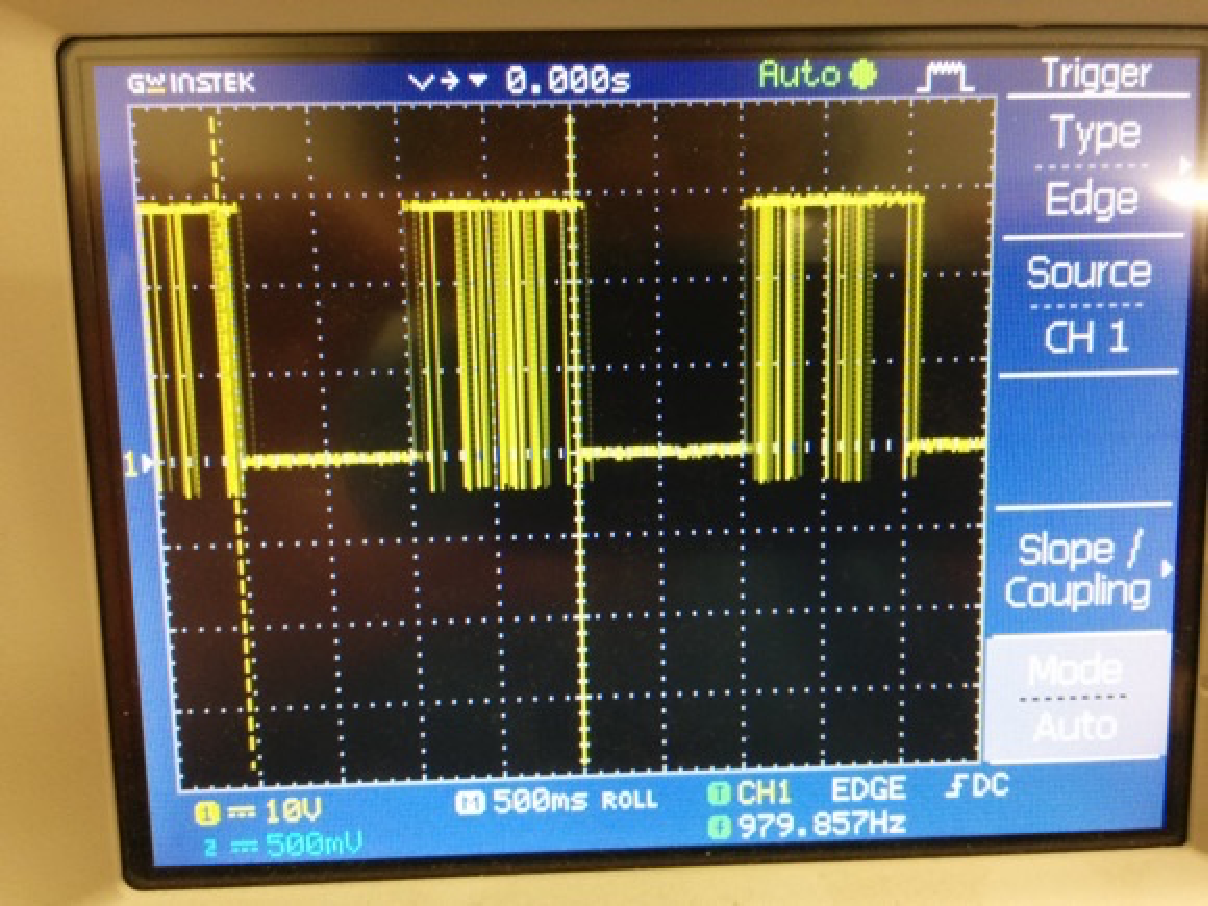
\includegraphics[width=110mm]{./image/out.pdf}
\caption{2SK2936からの出力}
\label{output}
\end{figure}

\begin{figure}[htbp]
\centering
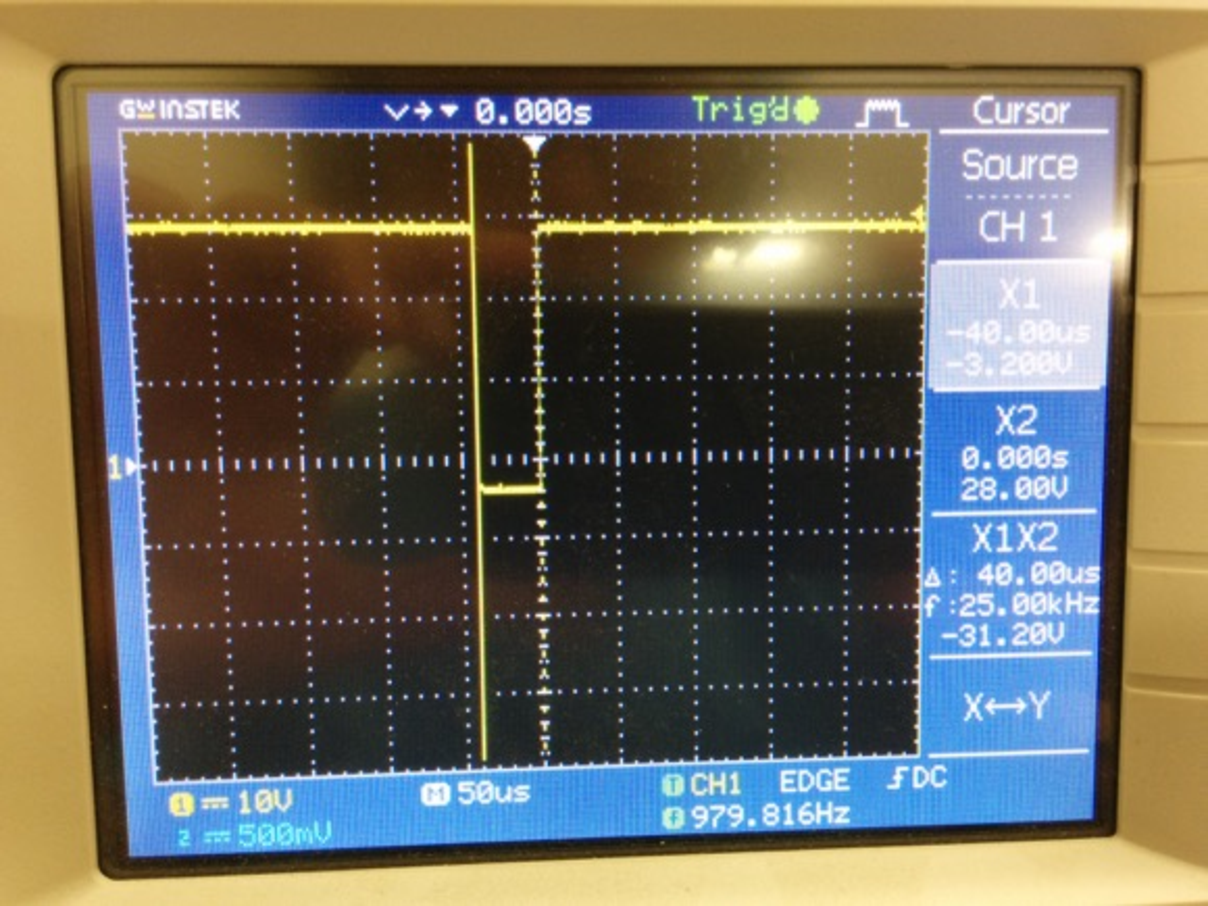
\includegraphics[width=110mm]{./image/short.pdf}
\caption{間欠ノイズの幅=40$\mu$s}
\label{short}
\end{figure}

\begin{figure}[htbp]
\centering
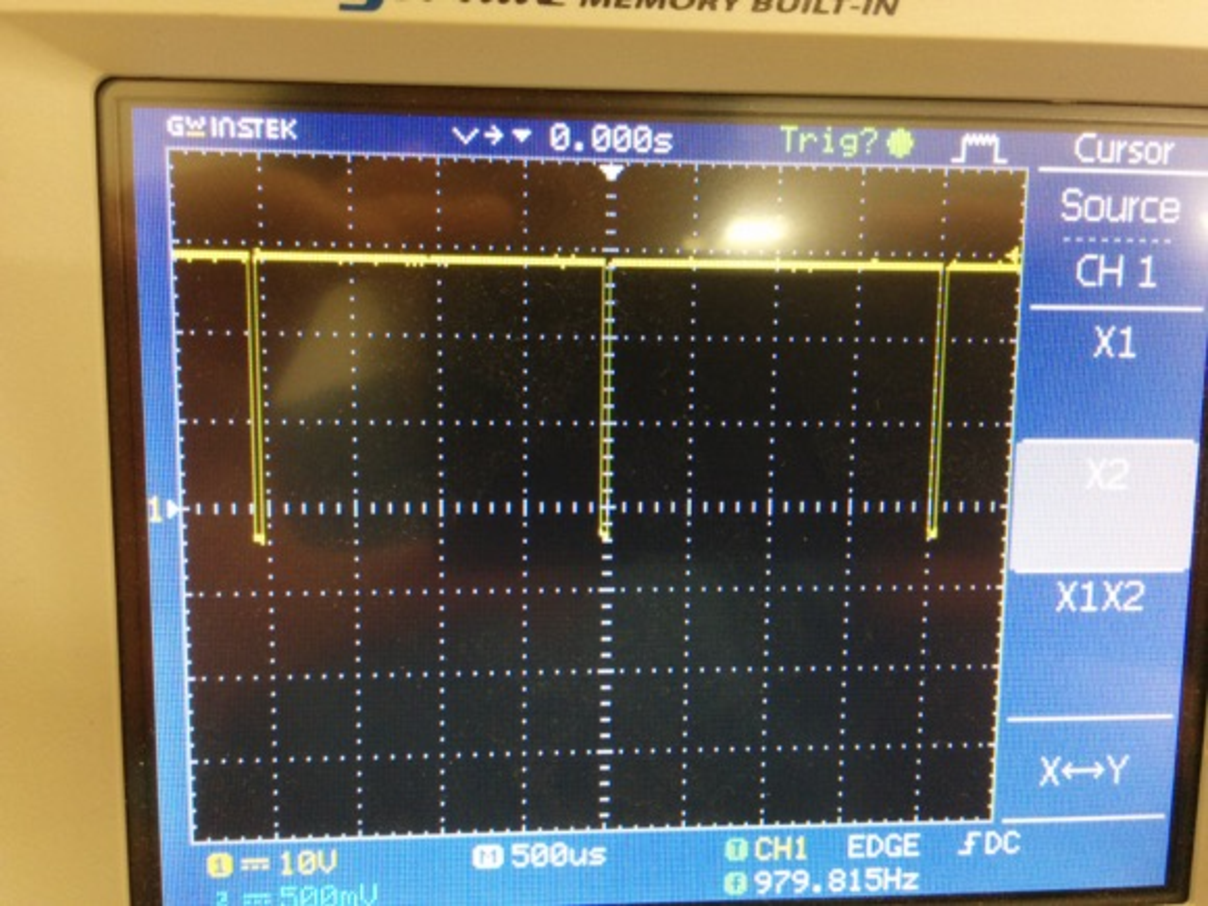
\includegraphics[width=110mm]{./image/long.pdf}
\caption{デューティ幅=2ms}
\label{long}
\end{figure}










\end{document}
